\begin{XeClass}{ChecksumFs}
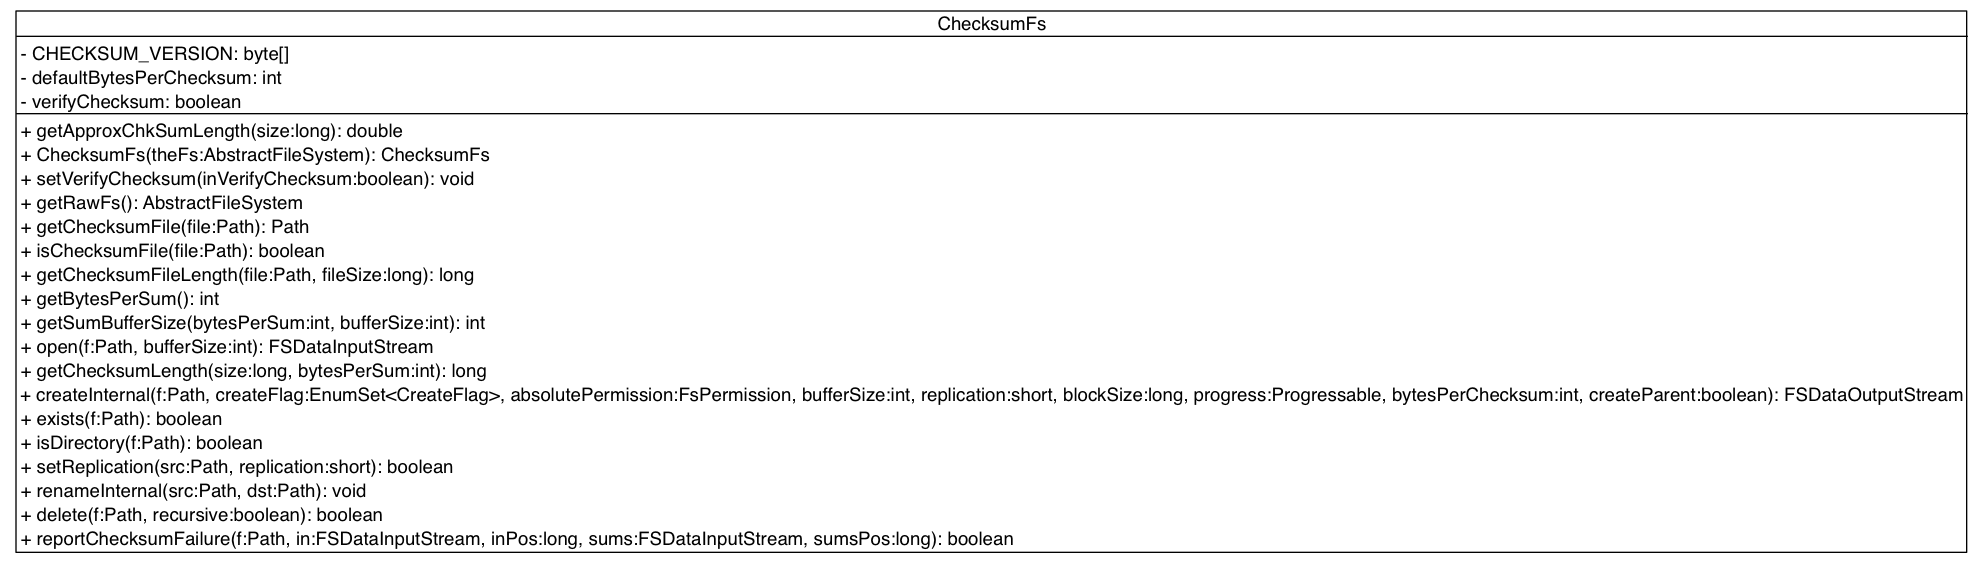
\includegraphics[width=10cm]{cdig/ChecksumFs.png}
     
 HDFS 会对写入的所有数据计算校验和(checksum),并在读取数据时验证校验和。
 针对指定字节的数目计算校验和。字节数默认是512 字节,可以通过io.bytes.per.checksum属性设置。
 通过CRC-32编码后为4字节。
 Datanode 在保存数据前负责验证checksum。
 client 会把数据和校验和一起发送到一个由多个datanode 组成的队列中,
 最后一个Datanode 负责验证checksum。
 如果验证失败,会抛出一个ChecksumException。客户端需要处理这种异常。
 客户端从datanode读取数据时,也会验证checksum。
 每个Datanode 都保存了一个验证checksum的日志。
 每次客户端成功验证一个数据块后,都会告知datanode,datanode会更新日志。
 每个datanode 也会在一个后台线程中运行一个DataBlockScanner,
 定期验证这个 datanode 上的所有数据块。
 在用Hadoop fs get命令读取文件时,可以用-ignoreCrc忽略验证。
 如果是通过FileSystem API 读取时,可以通过setVerifyChecksum(false),忽略验证。
 
 抽象检验文件系统 从文件系统过滤器类继承
 提供一个基本的文件校验系统的实现
 在客户端生成并且检验检验和,检验数据的完整性
 每个512byte的数据,生成一个4byte的检验和
 冗余备份的情况下,多个节点储存,以防止校验和本身损坏

    \begin{XeMethod}{\XePublic}{void}{setVerifyChecksum}
         
 布尔值 设置是否检验了校验和

    \end{XeMethod}

    \begin{XeMethod}{\XePublic}{AbstractFileSystem}{getRawFs}
         
 获取初始的文件系统

    \end{XeMethod}

    \begin{XeMethod}{\XePublic}{Path}{getChecksumFile}
         
 返回检验和文件关联文件的文件名

    \end{XeMethod}

    \begin{XeMethod}{\XePublic}{boolean}{isChecksumFile}
         
 当文件名是校验和文件名时,返回真值

    \end{XeMethod}

    \begin{XeMethod}{\XePublic}{long}{getChecksumFileLength}
         
 返回校验和文件的长度和源文件的大小

    \end{XeMethod}

    \begin{XeMethod}{\XePublic}{int}{getBytesPerSum}
         
 返回每个校验和的byte数

    \end{XeMethod}

    \begin{XeMethod}{\XePublic}{FSDataInputStream}{open}
         
 在指定的路径下开启一个FSData的输入流

    \end{XeMethod}

    \begin{XeMethod}{\XePublic}{long}{getChecksumLength}
         
 按byte计算校验和文件的长度

    \end{XeMethod}

    \begin{XeMethod}{\XePublic}{void}{renameInternal}
         
 重命名 files/dirs

    \end{XeMethod}

    \begin{XeMethod}{\XePublic}{boolean}{delete}
         
 在校验和文件系统中执行delete(Path, boolean)

    \end{XeMethod}

    \begin{XeMethod}{\XePublic}{boolean}{reportChecksumFailure}
         
 给文件系统报告一个校验和的错误

    \end{XeMethod}

    \begin{XeInnerClass}{ChecksumFSInputChecker}
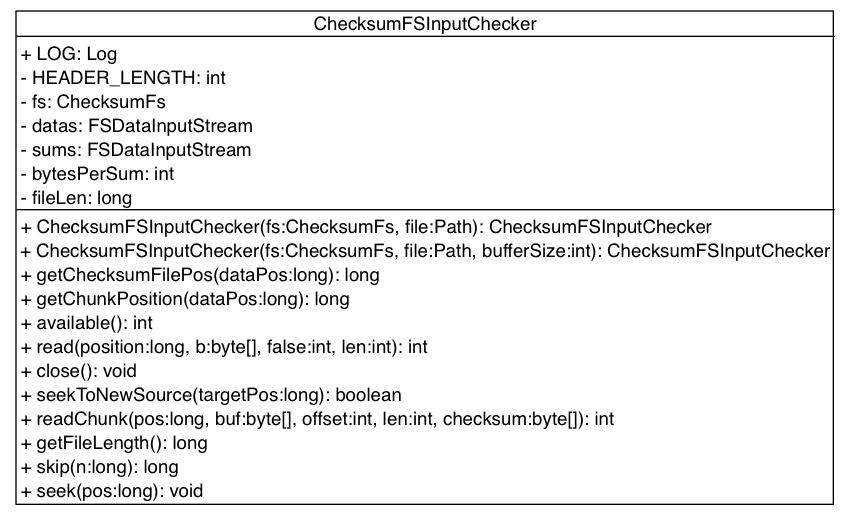
\includegraphics[width=10cm]{cdig/ChecksumFSInputChecker.png}
         
 open()方法的FS输入流
 确认数据和检验和是否匹配

        \begin{XeMethod}{\XePublic \\ \XeSync}{long}{skip}
             
 忽略或者弃用输入流中n byte的数据
 在总计忽略或者弃用n byte的数据前,用Skip方法忽略一些小的bytes
 实际忽略的byte数会被返回。如果n是负数,则不忽略任何byte。

        \end{XeMethod}

        \begin{XeMethod}{\XePublic \\ \XeSync}{void}{seek}
             
 在流中查找给定的位置
 下一次read()从此位置开始
 <p>此方法不允许搜索超过文件末,会抛出IOException

        \end{XeMethod}

    \end{XeInnerClass}
    \begin{XeInnerClass}{ChecksumFSOutputSummer}
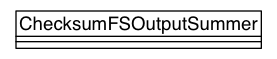
\includegraphics[width=10cm]{cdig/ChecksumFSOutputSummer.png}
         
 给校验过的文件提供一个输出流
 为数据生成检验和.

    \end{XeInnerClass}
\end{XeClass}
